Patient-generated longitudinal biomedical data is being produced at an increasing rate. These data are more dynamic and can better represent current patient health conditions. \phware\ is an effort to perform multidimensional analyses of such data to improve health outcomes by making patient-generated longitudinal data first-class data for creating a personalized, unified, coherent, and semantically-informed personalized data analyzer. Such an analyzer can be used in real-time by patients, and patient healthcare providers to improve the accuracy of diagnoses, treatments, and improve the overall quality of patient health at a lower cost.

\phware\ provides a wearable ring or finger-clip to measure vital signs. These devices are non-invasive, non-intrusive, and  communicate with a smartphone via Bluetooth using a simple application. The smartphone application uploads the sensor data to the \phware\ AI cloud services for storage and analysis. The AI cloud services performs an ensemble of algorithms and machine learning to increase the accuracy of values it assigns to vital signs [10-15]. Early accuracy validation for a consumer product version of \phware\ is within tolerance for medical use for oxygen saturation, respiration rate, temperature, heart rate/variability, and sys/diastolic blood pressures.

The \phware\ consumer product, assuming an eventual approval for medical application, is being explored as a means for remote patient monitoring systems as part of the short term and long term response to the COVID-19 global pandemic with the goal to improve the quality of healthcare services delivery at the point of care for COVID-19 outpatients. New development includes a highly usable web-based dashboard for providers to review vital sign trends and an alert for outpatients whose vital signs trends indicate elevated risk. 

\subsection{Conceptual Work Problem}
\begin{figure*}
  \begin{center}
    \begin{tabular}{c}
      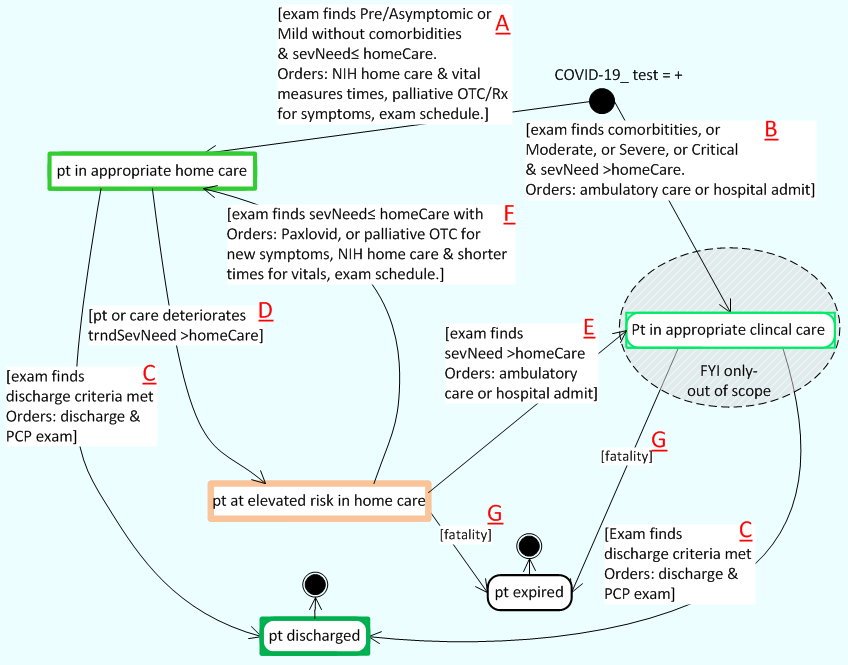
\includegraphics[scale=0.4]{cwp.png}
    \end{tabular}
  \end{center}
\caption{The CWP for remote COVID-19 patient care.}
\label{fig:cwp}
\end{figure*}

This expanded \phware\ system is modeled as a workflow using the \emph{Business Process Modeling Notation} (BPMN) [31]. Workflow modeling satisfies the need for effective functional integration of people and computing. A workflow is also able to preserve the medical decision authority of providers and enable the formal verification of the correctness of the end-to-end system design for outpatient safety.

The fundamental purpose of the expanded \phware\ system is to establish and maintain providers' timely awareness of outpatients' conditions and risk at home care, and thereby enhancing safety with better decisions to deliver more precise care. The concept is, however, abstract, intangible, and needs a more rigorous definition than common knowledge or intuition. 

This needed rigor is accomplished with a CWP, and the CWP becomes the verification requirement for the expanded \phware\ system that is used as a certification that the expanded system accomplishes its intended purpose of timely awareness and patient safety while in remote monitoring. This CWP is shown in \figref{fig:cwp}. 

As given in the introduction, a CWP [28-30] is a declarative specification of a complex object of work that is shared by activities in a distributed cognitive system. It makes clear the allowed transformations by the distributed activities to move the object from some initial state to a goal state. The specification provides a connection between human cognition and the design of a system such as \phware.

There are two parts to the CWP: the data defining the state of the object on the top left corner of \figref{fig:cwp}, and a state transition diagram, on the right of \figref{fig:cwp}, showing the allowed transitions between the object's states from some initial state to an eventual goal state. 

The object state adapts the Medicare 4-point severity-of-illness DRG ratings to represent the severity level of outpatient condition and their needed level of care [19, 20]. The ratings represent a composite of the CDC’s Interim Guidance for COVID-19 home care [46]. The adaptation here intends to capture the actionable risk awareness of a patient while in home care in a computationally independent model. 

The object state consists of the physician orders (\texttt{orders}), the actual severity of the patient on the 4-point scale (\texttt{sevLvl}), the level of care the patient is able to maintain, ether by caring for themselves or being cared for by a caregiver, while at home (\texttt{careCapLvl}), and the tending severity conjectured from the longitudinal data remotely being monitored and analyzed between exams as provided by the \phware\ AI cloud services (\texttt{trndSevLvl}).

The state transition diagram on the right of \figref{fig:cwp} shows the relevant care states with the associated risks patients can occupy and the transition conditions among them. In the initial state (top) the patient has tested positive. The arc labeled A occurs when an exam shows symptoms of low severity and a provider orders for home care with the expanded \phware\ system. 

Outpatients remain in appropriate home care until either an exam finds discharge criteria met and ordered (C), or trending severity level is greater than their care capability level (D). Is such cases, patients are at elevated risk. They must not remain at elevated risk in home care where there is a possible direct path to fatality (G). So an exam must either order admission (E), find their risk lower than what the analytics claimed, or make their risk lower with orders for better care at home. Patients who are admitted to hospital may eventually be discharged back to home care (H) or discharged directly (C). 

The declarative knowledge of the CWP specifies \emph{what} the \phware\ workflow design must accomplish without depending on \emph{how} it will be done. As such, it motivates the design, and then when the design is ready, the CWP is reused as the criterial property in formal verification to prove whether the \phware\ workflow satisfies the fundamental requirement to establish and maintain risk awareness. 

\subsection{Workflow Model}
\begin{figure*}
  \begin{center}
    \begin{tabular}{c}
      \includegraphics[scale=0.7]{bpmn.png}
    \end{tabular}
  \end{center}
\caption{The workflow model for the expanded \phware\ system.}
\label{fig:bpmn}
\end{figure*}

The workflow model for the expanded \phware\ system is in \figref{fig:bpmn}. It is designed with the MATH tool-suite [26] to model the functionality of interacting behaviors of the patient/caregiver, AI machine learning, and provider. MATH is an implementation of the BPMN standard with explicit representations for workflows performed by people and computing [31]. Applying and adapting BPMN to medical care and health informatics has become the focus of the recent BPM+ project within the Object Management Group [32]. 

The functional integration in the workflow model is adapted from concurrent design engineering in aerospace where there are specific tracks for each of multiple design disciplines that coordinate the work on a common physical design artifact [33]. The colored lanes of the workflow are the design tracks, and the CWP is the common work artifact that must be accomplished [26-30]. Each affects, and is affected, by the CWP. This feature is pivotal for integrating cognitive work that is distributed over people and computers. It allows people and computers to share work on the CWP despite vast differences in the performance properties of the way they do it. 

\figref{fig:bpmn} shows the workflow of patients, clinicians, \phware\ and other computer systems to establish and maintain risk awareness. It starts in the green clinician lane in the upper left of the workflow with a patient with a positive test. Such a positive test initiates an exam (task 01). The red letters indicate where the changes in the state of the CWP take place (i.e., the letters correspond to edges in the CWP). 

Hospital admission (task 03) corresponds to edges B and E in the CWP from \figref{fig:cwp}. A severity level less that two satisfies edges A and F with the workflow leading to the clinician orders for home care via \phware\ and tele-health exams augmented with realtime vitals (task 02). Discharge criteria include a second test with a negative result following the recovery period in clinic policy and cannot be met after the first exam.

The major part of the expanded \phware\ workflow begins in the bottom, salmon color, lane for the patient-caregiver. Task 04 obtains the \phware\ sensor and associated smartphone application. It then repeats recording vitals at provider-ordered time intervals (task 05) until an exam or expiration. The raw vitals data are transmitted by the smartphone application to the AI cloud services provided by \phware. 

The middle metallic grey lane represents the AI cloud services where the personal data analyzer operates on the data (task 06).  The analyzer immediately sends a packet to the clinician dashboard with vital sign values and trends for saturation, respiration rate, temperature, heart rate/variability, sys/diastolic blood pressures. An alert is added if the predicted trend exceeds home care capability or allowed severity in home care.

The specialized dashboard for clinicians’ maintains risk awareness for each outpatient (right side of the top green track). Alerts (task 07a) skip any routine delay for the provider’s attention. The workflow is designed to preserve the provider’s ultimate decision authority. The AI can reason that risk is elevated if it determines trending severity level is greater than home care capability level, and the provider can question the reasoning, and then confirm the alert or revise it. 

If an alert is confirmed, an urgent exam is ordered (task 08a) that is augmented by real-time vitals. An urgent exam may result in hospital admission (E in the CWP). When multiple patients have alerts, the provider must prioritize outpatients based on professional knowledge and patient familiarity. The provider may also decide the trend can be controlled by adjusting orders, such as more frequent vitals reporting or changing medications (F in the CWP). If an alert is dismissed by the provider, a routine exam still may be due to be scheduled (task 08b), or it may already be scheduled to start soon. 

For non-alerts, the provider reviews vitals when time permits (task 07b) and may order a routine exam to be scheduled. Alternatively, if clinical judgment deems it appropriate, the physician orders an urgent exam.
The decision gate 11 (far right of \figref{fig:bpmn}) is where exam times are managed. If an exam is already scheduled to begin soon the flow returns to task 01 where the next exam is held. The result of the exam is either to discharge, admit, or resume home care with remote monitoring and newly prescribed interventions as needed.

The rest of this paper describes the verification of the workflow against the CWP as a verification requirement. The verification is accomplished with the SPIN model checker. The CWP in \figref{fig:cwp} is translated into equivalent Linear Temporal Logic (LTL), and the workflow in \figref{fig:bpmn} in translated into its equivalent Promela model. The SPIN model checker then verifies the workflow to implement the CWP.
